\documentclass[10pt]{article}
\usepackage[utf8]{inputenc}
\usepackage[T1]{fontenc}
\usepackage{amsmath}
\usepackage{amsfonts}
\usepackage{amssymb}
\usepackage[version=4]{mhchem}
\usepackage{stmaryrd}
\usepackage{graphicx}
\usepackage[export]{adjustbox}
\graphicspath{ {./images/} }

\begin{document}
\section*{Math 141 Tutorial 1}
\section*{Main problems}
\begin{enumerate}
  \item Compute the following sums and simplify your answer to a single number\\
(a) $\sum_{i=-2}^{2}(2 i+1)$\\
(d) $\sum_{i=2}^{5} \frac{i^{2}-2 i+1}{i-1}$\\
(b) $\sum_{i=-2}^{2} 2 i+1$\\
(e) $\sum_{i=-1}^{1} 2^{i}$\\
(c) $\sum_{i=1}^{4} \frac{1}{i}+1$\\
(f) $\sum_{i=1}^{4} \log _{24} i$
  \item Using Riemann sums with $n$ subintervals, approximate the area under the following curves. Draw a picture in order to visualize the rectangles whose areas are being summed.\\
(a) With $n=4$ and either left or right Riemann sums, approximate the area under the curve of $f(x)=2 x-4$ from $x=2$ to $x=4$. What is the true area?\\
(b) With $n=4$ and both left and right Riemann sums, approximate the area under $f(x)=x^{3}$ from $x=0$ to $x=2$. By using both left and right Riemann sums, one obtains upper and lower bounds for the true area. Which method gives a lower bound on the true area? How do you explain this?\\
(c) What do you expect to happen if we repeat the process in part (b) with $n=6$ ? Should we be closer or further from the "true area"?
  \item For each function $f(x)$ and interval, write the Riemann sum that approximates the area under the curve for any $n \geq 1$.\\
(a) The area under $f(x)=2 x$ between $x=0$ and $x=2$\\
(b) The area between $f(x)=-x+3$, the x -axis and the lines $x=1$ and $x=4$\\
(c) The area under $f(x)=2 x^{2}+1$ between $x=0$ and $x=2$
  \item We tackle now the inverse process: for each of the following Riemann sums find a function $f(x)$ and values $a$ and $b$ such that the limit expresses the area above/below $f(x)$ between $x=a$ and $x=b$.
\end{enumerate}

Note: There may be several valid answers for each problem.\\
Hint: Every sum appearing in this problem can be realized as a right Riemann sum.\\
(a) $\sum_{i=1}^{n}\left(\frac{3 i}{n}-3\right) \frac{3}{n}$\\
(b) $\sum_{i=1}^{n} \frac{\left(2+\frac{i}{n}\right)^{2}+\left(2+\frac{i}{n}\right)}{n}$\\
(c) $\sum_{i=1}^{n} e^{\frac{6 i}{n}-2} \frac{6}{n}$\\
(d) $\sum_{i=1}^{n}\left(\frac{3 i}{2 n}+\frac{1}{2}\right) \tan \left(\frac{3 i}{2 n}-\frac{3}{2}\right) \frac{3}{2 n}$

\section*{Challenge problems}
\begin{enumerate}
  \setcounter{enumi}{4}
  \item Using a combination of left and right Riemann sums with $n=4$, find both an upper and lower bound for the area under $f(x)=2 x-x^{2}$ from $x=0$ to $x=2$.
  \item Another method for approximating the area under a curve is known as the Trapezoidal Rule. Here, instead of using rectangles, trapezoids are used. The area of the trapezoid below $f(x)$ and between the nodes $x_{i}$ and $x_{i+1}$ is given by\\
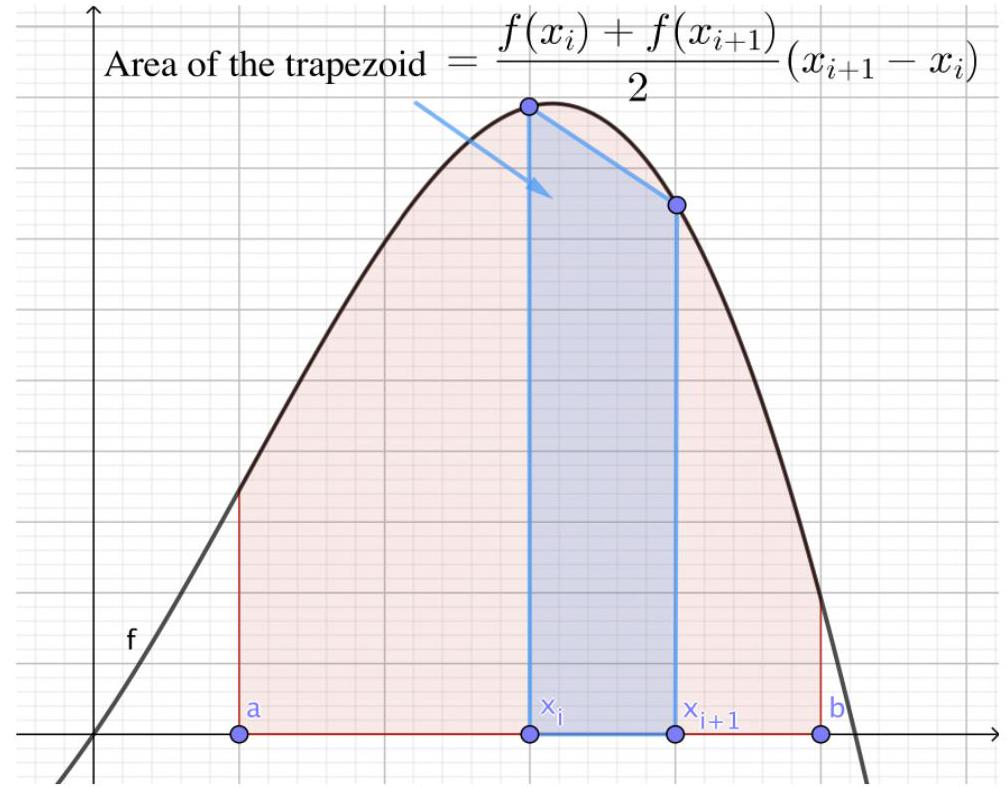
\includegraphics[max width=\textwidth, center]{2024_12_27_b6d734ff7fda15966c90g-6}\\
(a) Write down an equation for the Trapezoidal Rule when using a fixed number $n$ of trapezoids to approximate the area under $f(x)$ between $x=a$ and $x=b$.\\
(b) Can you write down the formula for the Trapezoidal Rule in terms of left and right Riemann sums?
\end{enumerate}

\end{document}